\documentclass[a4paper,12pt]{article}
\usepackage{hyperref}
\usepackage{fullpage}
\usepackage{caption}
\usepackage{subcaption}
\usepackage{url}
\usepackage{graphicx}
\usepackage{hyperref}
\usepackage{listings}
\usepackage{color}
\usepackage{listings}
\usepackage{color}
\usepackage{amsmath}
\usepackage{amssymb}


\author{Paul Rubenstein\\ \texttt{pkr235@cam.ac.uk} \and Steve Smith \\ \texttt{sps41@cam.ac.uk} \and Argyris Zardilis \\ \texttt{az325@cam.ac.uk}}
\title{Systems Biology Assignment}

\begin{document}
\maketitle

\section*{Question 1}
\subsection*{A}
\[f(x) = \lambda \frac{K^n}{K^n + x^n}\]
\underline{Claim:} The log-log sensitivity of $f(x)$ is bounded (below) by $-n$.

\noindent \underline{Proof:} 
\begin{align*}
\frac{\partial \ln f}{\partial \ln x} & =  \frac{\partial f(x)}{\partial x}\frac{x}{f(x)} \\
& = \frac{\partial (\lambda \frac{K^n}{K^n + x^n})}{\partial x} \frac{x(K^n + x^n)}{\lambda K^n} \\
& = \frac{- \lambda K^n n x^{n-1}}{(K^n + x^n)^2} \frac{x(K^n + x^n)}{\lambda K^n} \\
& = \frac{-n x^n}{K^n + x^n}\\
& = -n \cdot \frac{1}{(K/x)^n+1}
\end{align*}

Now $K, x, n \geq 0$ and hence the denominator in the preceeding line is larger than 1. Thus:

\begin{align*}
\frac{\partial \ln f}{\partial \ln x} & = -n \cdot \frac{1}{(K/x)^n+1} \geq -n
\end{align*}

And thus the claim is true. $\square$

For an example plot of a Hill-type repression function, see Figures \ref{hill} and \ref{log-log}. Note that the log-log sensitivity tends to $-1$ as $x\longrightarrow \infty$

\begin{figure}
\centering
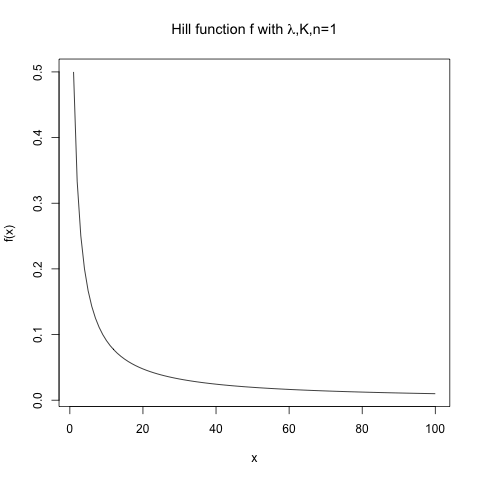
\includegraphics[width=5in]{images/hill.png}
\caption{A plot of the Hill function $f(x) = \lambda \frac{K^n}{K^n+x^n}$}
\label{hill}
\end{figure}

\begin{figure}
\centering
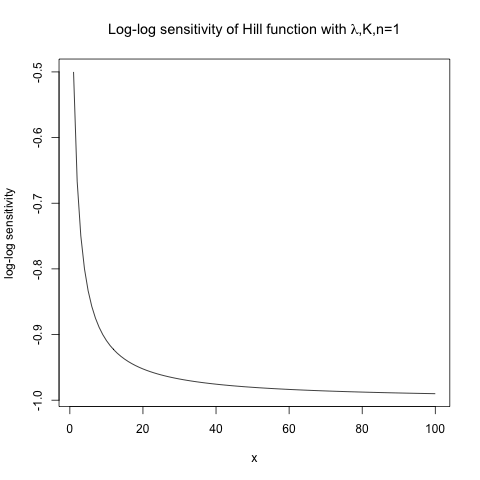
\includegraphics[width=5in]{images/log-log.png}
\caption{Log-log sensitivity of the Hill function $f(x) = \lambda \frac{K^n}{K^n+x^n}$. Note that the curve tends to $-1$ as $x\longrightarrow \infty$}
\label{log-log}
\end{figure}

\subsection*{B}

\underline{Claim:} \[f(x) = a x+b \Rightarrow \left \langle \frac{\Delta f / \langle f \rangle}{\Delta x / \langle x \rangle}  \frac{{\Delta x}^2}{\langle \Delta x^2 \rangle} \right \rangle = \frac{\partial \ln f}{\partial \ln x} \bigg|_{x=\langle x \rangle} \]

\noindent \underline{Proof:}

\[ \frac{\partial \ln f}{\partial \ln x} \bigg|_{x=\langle x \rangle} = \frac{\partial f}{\partial x} \frac{x}{f} \bigg|_{x=\langle x \rangle} = \frac{a\langle x \rangle}{a \langle x \rangle + b}\]

and

\[ \Delta f = f - \langle f \rangle = (ax+b) - (a \langle x \rangle - b) = a \Delta x\]

Thus:

\begin{align*}
\left \langle \frac{\Delta f / \langle f \rangle}{\Delta x / \langle x \rangle} \frac{{\Delta x}^2}{\langle \Delta x^2 \rangle} \right \rangle & = \left \langle \frac{a \Delta x /( a \langle x \rangle - b)}{\Delta x / \langle x \rangle} \frac{\Delta x ^2}{\langle \Delta x ^2 \rangle} \right \rangle \\
&= \left \langle \frac{a \langle x \rangle}{a \langle x \rangle - b} \frac{\Delta x ^2}{\langle \Delta x ^2 \rangle} \right \rangle \\
&= \frac{a \langle x \rangle}{a \langle x \rangle - b} \frac{\langle \Delta x ^2 \rangle}{\langle \Delta x ^2 \rangle} = \frac{a \langle x \rangle}{a \langle x \rangle - b} = \frac{\partial \ln f}{\partial \ln x} \bigg|_{x=\langle x \rangle}
\end{align*}

Since $a, \langle x \rangle$ and $\langle \Delta x^2\rangle$ are constants. Thus the claim is true.  $\square$

\subsection*{C}

The difference between the two corrective measures - the overall corrective tendency and the log-log sensitivity - is that the former is `the true behaviour of the system' whereas the latter is used as an approximation to the former as it is easier to calculate and use in analysis. Part B above shows that in the case that $f$ is a linear function of $x$, the two quantities are equal. If $f$ is well-behaved near the stationary value for $x$ and the fluctuations are small we can approximate $f$ by a linear function of $x$ by Taylor's theorem. Thus we can use $\frac{\partial \ln f}{\partial \ln x}$ as a valid approximation to the true corrective function in this case.


\section*{Question 2}

\end{document}